\documentclass[11pt]{article}
\usepackage[usenames, dvipsnames]{color}
\usepackage[margin=1in,vmargin=1in]{geometry}
\usepackage[utf8]{inputenc}
\usepackage[english]{babel}
\usepackage{tikz}
\usepackage{pgfplots}
\usepackage{fancyhdr}
\usepackage{comment}
\pagestyle{fancy}
\usepackage{url}
\usepackage[font=small,labelfont=bf,labelsep=period]{caption}
\usepgfplotslibrary{polar}
\usepgflibrary{shapes.geometric}
\usetikzlibrary{calc}
\pgfplotsset{compat=1.5.1}
\pgfmathdeclarefunction{gauss}{2}{%
  \pgfmathparse{1/(#2*sqrt(2*pi))*exp(-((x-#1)^2)/(2*#2^2))}%
}

\pgfmathdeclarefunction{bivar}{4}{%
  \pfgmathparse{1/(2*pi*#2*#4) * exp(-((x-#1)^2/#2^2 +
    (y-#3)^2/#4^2))/2}%
}
\usetikzlibrary{shadows}
\usepackage{graphicx}
\usepackage{graphics}
\usepackage[mode=buildnew]{standalone}
\usepackage{amsmath}
\usepackage{amsthm}
\usepackage{amssymb}
\usepackage{float}
\usepackage{hyperref}
\DeclareMathOperator*{\argmin}{arg\,min}
\newcommand*{\everymodeprime}{\ensuremath{\prime}}
\graphicspath{{figs/}}

\title{Label Smoothing with Graph Convolution}
\author{}
\date{}

\begin{document}

\maketitle

\section{Graph Convolution}

Most algorithms seem to be doing variants of the same general algorithm. I think it is a good exercise for me to go through some of these papers and explain how they related to each other in the context of probabilistic modeling. The goal is to clearly outline the relationships among these different algorithms to more clearly see a way to contribute to this area.

% table comparing methods in papers. for example, organize the more recent publications on the clothing1m dataset into a table
% identify the top noisy label/label smoothing papers
% graphconv + knn + update (main idea); run a simple algorithm on mnist
% 

\vspace{2cm}
\noindent Some take-aways from reading papers thus far
\begin{itemize}
\item It seems that utilizing information during the learning process is a younger/current research area with some room to publish. That seems promising for us using GraphConvolution to regularize the deep learning model
\item I think using GraphConv to regularize the loss function would be analogous to some type of ``perceptual loss'' function people use currently. I think we would have to compare to ``regularized classification'' methods as well, rather than just ``noisy labels'' papers. I think it is \emph{very popular} to use the final representations of a neural network to inform some part of learning or testing. I think we need to widen the related literature scope to understand if we are calling ``noisy labels'' by the wronge name; e.g. simply training to find good representations implies we perform the same algorihm as our proposed one. This means we would taking PAPER X's algorithm (ALG X) and applying it to ``noisy labels'' (APPLICATION Y) and our contribution would be limited to (i) identifying ALG X can be applied to APPLICATION Y and (ii) maybe providing some justifiction for such appilcations. Is this enough of a paper? This seems weak to me.
\end{itemize}

\vspace{2cm}
\noindent Other tasks I am looking to complete are:
\begin{itemize}
\item Code up some Graph convolution (complete)
\item Understand how collaborative filtering relates to markov random fields
\end{itemize}

\begin{figure}[h]
  \centering
  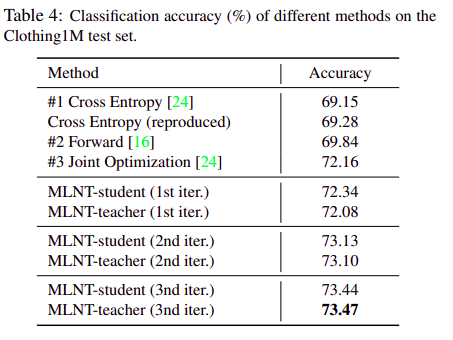
\includegraphics[width=0.5\linewidth]{cvpr2019_learning_to_learn_w_noisy_data}
  \caption{Clothing 1M Result from cvpr2019 ``learning to learn with noisy data''. Ref 24 is cvpr2018 ``Joint optimization framework for learning with noisy labels.'' Ref 16 is cvpr 2017 ``Making deep neural networks robust to label noise: A loss correction approach.''}
\end{figure}

\begin{figure}[h]
  \centering
  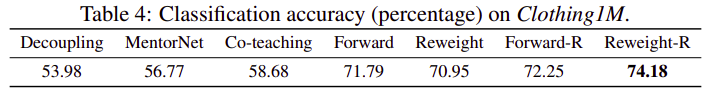
\includegraphics[width=0.8\linewidth]{neurips2019_anchor_points}
  \caption{Clothing 1M Result from neurips2019 ``Are Anchor Points Really Indispensable in Label-Noise Learning?''. neurips 2018 ``Decoupling'' = ``Decoupling "when to update" from "how to update"... }
\end{figure}


\clearpage
\newpage
\section{References}
\noindent {\bf Are Anchor Points Really Indispensable in Label-Noise Learning?}

\noindent NeurIPs 2019

\noindent Citations: 6

\noindent Url: \url{https://arxiv.org/pdf/1906.00189.pdf}

\begin{itemize}
   \item Risk and Classification statistically consistent methods rely on transition matrices. 
   \item Existing theories have shown that the transition matrix can be learned by exploiting anchor points
   \item when there are no anchor points, the transition matrix will be poorly learned
   \item without employing anchor points, we propose a transition-revision (T-Revision) method to effectively learn transition matrices
   \item we first initialize it by exploiting data points that are similar to anchor points, having high noisy class posterior probabilities. Then, we modify the initialized matrix by adding a slack variable, which can be learned and validated together with the classifier by using noisy data
\end{itemize}

\vspace{2cm}\noindent {\bf Combinatorial Inference against Label Noise}

\noindent NeurIPs 2019

\noindent Citations: 0

\begin{itemize}
  \item a unique classification framework of constructing multiple models in heterogeneous coarse-grained meta-class spaces and making joint inference of the trained models for the final predictions in the original (base) class space.
  \item improvement via constructing meta-classes and improves accuracy via combinatorial inferences over multiple constituent classifiers
  \item distinct and complementary properties for the given problem, we can even incorporate additional off-the-shelf learning algorithms to improve accuracy further
  \item techniques to organize multiple heterogeneous meta-class sets using k-means clustering and identify a desirable subset leading to learn compact models
\end{itemize}

\vspace{2cm}\noindent {\bf L\_DMI: A Novel Information-theoretic Loss Function for Training Deep Nets Robust to Label Noise}

\noindent NeurIPs 2019

\noindent Citations: 6

\begin{itemize}
  \item most methods only handle limited kinds of noise patterns, require auxiliary information or steps (e.g., knowing or estimating the noise transition matrix), or lack theoretical justification. 
  \item novel information-theoretic loss function, LDMI, for training deep neural networks robust to label noise
  \item generalized version of mutual information, termed Determinant based Mutual Information (DMI), which is not only information-monotone but also relatively invariant.
  \item provably robust to instance-independent label noise, regardless of noise pattern, and it can be applied to any existing classification neural networks straightforwardly without any auxiliary information
\end{itemize}


\vspace{2cm}\noindent {\bf Robust Inference via Generative Classifiers for Handling Noisy Labels}

\noindent ICML 2019

\noindent Citations: 7

\noindent Url: \url{https://arxiv.org/pdf/1901.11300.pdf}

\begin{itemize}
  \item induce a generative classifier on top of hidden feature spaces of the pre-trained DNNs, for obtaining a more robust decision boundary
  \item By estimating the parameters of generative classifier using the minimum covariance determinant estimator, we significantly improve the classification accuracy with neither re-training of the deep model nor changing its architectures
  \item assumption of Gaussian distribution for features, we prove that RoG generalizes better than baselines under noisy labels.
  \item we propose the ensemble version of RoG
\end{itemize}


\vspace{2cm}\noindent {\bf Unsupervised Label Noise Modeling and Loss Correction}

\noindent ICML 2019

\noindent Citations: 13

\noindent Url: \url{https://arxiv.org/pdf/1904.11238.pdf}

\begin{itemize}
  \item two-component mixture model as an unsupervised generative model of sample loss values during training to allow online estimation of the probability that a sample is mislabelled. 
  \item beta mixture to estimate this probability and correct the loss by relying on the network prediction (the so-called bootstrapping loss).
  \item We further adapt mixup augmentation to drive our approach a step further; mixing two classes in raw pixel space
\end{itemize}

\vspace{2cm}\noindent {\bf How does Disagreement Help Generalization against Label Corruption?}

\noindent ICML 2019

\noindent Citations: 18

\vspace{2cm}\noindent {\bf Learning to Learn from Noisy Labeled Data}

\noindent CVPR 2019

\noindent Citations: 26

\noindent Tags: learning dynamics

\noindent Url: \href{https://arxiv.org/pdf/1812.05214.pdf}{url}

\begin{itemize}
  \item meta-learning update is performed prior to conventional gradient update.
  \item proposed meta-learning method simulates actual training by generating synthetic noisy labels, and train the model such that after one gradient update using each set of synthetic noisy labels
\end{itemize}

\vspace{2cm}\noindent {\bf Co-teaching: Robust Training of Deep Neural Networks with Extremely Noisy Labels}

\noindent NeurIPs 2018

\noindent Citations: 130

\noindent Url: \href{https://arxiv.org/pdf/1804.06872.pdf}{url}

\begin{itemize}
\item first memorize training data of clean labels and then those of noisy labels
\item a new deep learning paradigm called “Co-teaching” for combating with noisy labels
\item we train two deep neural networks simultaneously, and let them teach each other given every mini-batch:
\item firstly, each network feeds forward all data and selects some data of possibly clean labels
\item  secondly, two networks communicate with each other what data in this mini-batch should be used for training;
\item finally, each network back propagates the data selected by its peer network and updates itself
\end{itemize}

\vspace{2cm}\noindent {\bf Robustness of conditional GANs to noisy labels}

\noindent NeurIPs 2018

\noindent Citations: 17

\noindent Url: \href{https://papers.nips.cc/paper/8229-robustness-of-conditional-gans-to-noisy-labels.pdf}{url}

\begin{itemize}
  \item learning conditional generators from noisy labeled samples, where the labels are corrupted by random noise
  \item standard training of conditional GANs will not only produce samples with wrong labels, but also generate poor quality samples
  \item We consider two scenarios, depending on whether the noise model is known or not.
  \item known noise: introduce a novel architecture RCGAN. The main idea is to corrupt the label of the generated sample before feeding to the adversarial discriminator, forcing the generator to prouce samples with clean labels
  \item unknown noise: we provide an extension of our architecture, which we call RCGAN-U
\end{itemize}

\vspace{2cm}\noindent {\bf Masking: A New Perspective of Noisy Supervision}

\noindent NeurIPs 2018

\noindent Citations: 30

\begin{itemize}
  \item corruption of labels via unknown noise transition matrix.
  \item by estimating this matrix, classifiers can escape from overfitting those noisy labels. such estimation is practically difficult
  \item human-assisted approach called “Masking” that conveys human cognition of invalid class transitions and naturally speculates the structure of the noise transition matrix
  \item structure-aware probabilistic model incorporating a structure prior, and solve the challenges from structure extraction and structure alignment
  \item only estimate unmasked noise transition probabilities and the burden of estimation is tremendously reduced
\end{itemize}

\vspace{2cm}\noindent {\bf Robust training of deep neural networks with extremely noisy labels.}

\noindent NeurIPs 2018

\noindent Citations: 130

\vspace{2cm}\noindent {\bf Using Trusted Data to Train Deep Networks on Labels Corrupted by Severe Noise}

\noindent NeurIPs 2018

\noindent Citations: 77

\begin{itemize}
\item previous works assume that no source of labels can be trusted. 
\item we relax this assumption and assume that a small subset of the training data is trusted
\item substantial label corruption robustness performance gains.
\item particularly severe label noise can be combated by using a set of trusted data with clean labels.
\end{itemize}

\noindent comments:
\begin{itemize}
\item this seems closest to the mrf model
\end{itemize}

\vspace{2cm}\noindent {\bf Generalized Cross Entropy Loss for Training Deep Neural Networks with Noisy Labels}

\noindent NeurIPs 2018

\noindent Citations: 150

\noindent Url: \href{https://papers.nips.cc/paper/8094-generalized-cross-entropy-loss-for-training-deep-neural-networks-with-noisy-labels.pdf}{url}

\begin{itemize}
\item mean absolute error (MAE) has recently been proposed as a noise-robust alternative to the commonly-used categorical cross entropy (CCE) loss.
\item shown here, MAE can perform poorly with DNNs and challenging datasets
\item we present a theoretically grounded set of noise-robust loss functions that can be seen as a generalization of MAE and CCE.
\end{itemize}

\vspace{2cm}\noindent {\bf Robot Learning in Homes: Improving Generalization and Reducing Dataset Bias}

\noindent NeurIPs 2018

\noindent Citations: 25

\begin{itemize}
\item data collected using low cost robots suffer from noisy labels due to imperfect execution and calibration errors.
\item To handle this, we develop a framework which factors out the noise as a latent variable
\item Use direct optimization to learn join of $p(\hat{y},y|x)$ from Misera 2015.
\end{itemize}

\vspace{2cm}\noindent{\bf Masking: A new perspective of noisy supervision.}

\noindent NeurIPs 2018

\noindent Citations: 30

\vspace{2cm}\noindent {\bf Learning to Reweight Examples for Robust Deep Learning}

\noindent ICML 2018

\noindent Citations: 162

\noindent Url: \href{https://arxiv.org/pdf/1803.09050.pdf}{url}

\begin{itemize}
  \item learns to assign weights to training examples based on their gradient directions.
  \item meta gradient descent step on the current mini-batch example weights (which are initialized from zero) to minimize the loss on a clean unbiased validation set.
  \item an any type of deep network, does not require any additional hyperparameter tuning
  \item on class imbalance and corrupted label problems where only a small amount 
\end{itemize}

\begin{itemize}
\item They use the same latent space representation of the real label as I do
\end{itemize}

\vspace{2cm}\noindent {\bf MentorNet: Learning Data-Driven Curriculum for Very Deep Neural Networks on Corrupted Labels}

\noindent ICML 2018

\noindent Citations: 189

\noindent Tags:


\vspace{2cm}\noindent {\bf Dimensionality-Driven Learning with Noisy Labels}

\noindent ICML 2018

\noindent Citations: 75

\noindent Tags: learning dynamics

\begin{itemize}
\item a new perspective for understanding DNN generalization for such datasets, by investigating the dimensionality of the deep representation subspace of training samples
\item from a dimensionality perspective, DNNs exhibit quite distinctive learning styles when trained with clean labels versus when trained with a proportion of noisy labels
\item a new dimensionality-driven learning strategy, which monitors the dimensionality of subspaces during training and adapts the loss function accordingly
\end{itemize}

\vspace{2cm}\noindent {\bf Learning with biased complementary labels}

\noindent ICCV/ECCV 2018

\noindent Citations: 47

\vspace{2cm}\noindent {\bf Curriculumnet: Weakly supervised learning from large-scale web images.}

\noindent ICCV/ECCV 2018

\noindent Citations: 26

\vspace{2cm}\noindent {\bf Exploring the Limits of Weakly Supervised Pretraining}

\noindent ICCV/ECCV 2018

\noindent Citations: 229

\begin{itemize}
\item DNN trained to predict hashtags on billions of social media images.
\item not really noisy labels
\end{itemize}

\vspace{2cm}\noindent {\bf CurriculumNet: Weakly Supervised Learning from Large-Scale Web Images}

\noindent ICCV/ECCV 2018

\noindent Citations: 47

\begin{itemize}
\item We develop a principled learning strategy by leveraging curriculum learning, with the goal of handling a massive amount of noisy labels and data imbalance effectively.
\item measuring the complexity of data using its distribution density in a feature space, and rank the complexity in an unsupervised manner.
\item where the negative impact of noisy labels is reduced substantially
\item highly noisy labels can improve testing accuracy by serving as regularization
\end{itemize}

\vspace{2cm}\noindent {\bf Deep Learning is Robust to Massive Label Noise (rejected from iclr 2018; referenced in iclr 2019 reject as "worth reading")}

\noindent ICLR 2018

\noindent Citations: 145

\begin{itemize}
\item show deep neural networks are capable of generalizing from training data for which true labels are massively outnumbered by incorrect labels.
\item demonstrate remarkably high test performance after training on corrupted data from MNIST, CIFAR, and ImageNet.
\item For example, on MNIST we obtain test accuracy above 90 percent even after each clean training example has been diluted with 100 randomly labeled examples.
\item We show that training in this regime requires a significant but manageable increase in dataset size that is related to the factor by which correct labels have been diluted.
\item a result shows how increasing noise decreases the effective batch size.
\end{itemize}

\vspace{2cm}\noindent {\bf Learning From Noisy Singly-labeled Data}

\noindent ICLR 2018

\noindent Citations: 43

\begin{itemize}
\item how to optimally learn from multiple noisy workers?
\item how to allocate labeling budget to maximum classifier performance?
\item propose a new algorithm for jointly modeling labels and worker quality from noisy crowd-sourced data
\item alternating minimization proceeds in rounds, estimating worker quality from disagreement with the current model and then updating the model by optimizing a loss function that accounts for the current estimate of worker quality. (EM algorithm)
\item even with only one annotation per example, our algorithm can estimate worker quality.
\end{itemize}

\vspace{2cm}\noindent {\bf Robust active label correction}

\noindent AISTAT 2018

\noindent Citations: 5

\vspace{2cm}\noindent {\bf Joint Optimization Framework for Learning With Noisy Labels}

\noindent CVPR 2018

\noindent Citations: 96

\begin{itemize}
\item 
\end{itemize}

\vspace{2cm}\noindent {\bf Iterative Learning With Open-Set Noisy Labels}

\noindent CVPR 2018

\noindent Citations: None

\vspace{2cm}\noindent {\bf CleanNet: Transfer Learning for Scalable Image Classifier Training With Label Noise}

\noindent CVPR 2018

\noindent Citations: None

\vspace{2cm}\noindent {\bf Detection and Correction of Mislabeled Training Samples for Hyperspectral Image Classification}

\noindent GRS 2018

\noindent Citations: None

\vspace{2cm}\noindent {\bf On the Resistance of Nearest Neighbor To Random Noisy Labels (reference by reviewer when rejecting iclr 2019 paper)}

\noindent ??? 2018

\noindent Citations: None

\vspace{2cm}\noindent {\bf Toward Robustness against Label Noise in Training Deep Discriminative Neural Networks}

\noindent NeurIPs 2017

\noindent Citations: 87

\vspace{2cm}\noindent {\bf Decoupling "when to update" from "how to update"}

\noindent NeurIPs 2017

\noindent Citations: 63

\vspace{2cm}\noindent {\bf Learning from noisy labels with distillation.}

\noindent ICCV/ECCV 2017

\noindent Citations: 147

\vspace{2cm}\noindent {\bf Revisiting Unreasonable Effectiveness of Data in Deep Learning Era}

\noindent ICCV/ECCV 2017

\noindent Citations: 430

\vspace{2cm}\noindent {\bf Learning From Noisy Large-Scale Datasets With Minimal Supervision}

\noindent CVPR 2017

\noindent Citations: None

\vspace{2cm}\noindent {\bf Making Deep Neural Networks Robust to Label Noise: A Loss Correction Approach}

\noindent CVPR 2017

\noindent Citations: None

\vspace{2cm}\noindent {\bf Robust Loss Functions under Label Noise for Deep Neural Networks}

\noindent AAAI 2017

\noindent Citations: None

\vspace{2cm}\noindent {\bf Learning with Confident Examples: Rank Pruning for Robust Classification with Noisy Labels}

\noindent UAI 2017

\noindent Citations: None

\vspace{2cm}\noindent {\bf Effect of Training Class Label Noise on Classification Performances for Land Cover Mapping with Satellite Image Time Series}

\noindent MDPI 2017

\noindent Citations: None

\vspace{2cm}\noindent {\bf The Unreasonable Effectiveness of Noisy Data for Fine-Grained Recognition}

\noindent ICCV/ECCV 2016

\noindent Citations: 219

\vspace{2cm}\noindent {\bf Learning Visual Features from Large Weakly Supervised Data}

\noindent ICCV/ECCV 2016

\noindent Citations: 143

\vspace{2cm}\noindent {\bf Seeing through the Human Reporting Bias: Visual Classifiers from Noisy Human-Centric Labels}

\noindent CVPR 2016

\noindent Citations: 86

\begin{itemize}
\item for a choice of what object to assign an image, workers use subjective judgement. noisy “human-centric” annotations as exhibiting human reporting bias.
\item use these noisy annotations for learning visually correct image classifiers.
\item  Such annotations do not use consistent vocabulary, and miss a significant amount of the information present in an image
\item we demonstrate that the noise in these annotations exhibits structure and can be modeled.
\item an algorithm to decouple the human reporting bias from the correct visually grounded labels
\item highly interpretable for reporting “what’s in the image” versus “what’s worth saying.”
\item uses latent indicator function $z$ to say ``person image not person image?'' to estimate the distribution of the ``relevent'' objects in the image. This is pretty hand-wavey and relies on learning the conditional estimates $z$ and the ``visually grounded predicitons'' classifier...
\end{itemize}

\noindent comments
\begin{itemize}
\item written to personify estimating parametric functions: ``see through''. ew lol
\end{itemize}

\vspace{2cm}\noindent {\bf Learning with Noisy Labels}

\noindent NeurIPs 2015

\noindent Citations: 483

\vspace{2cm}\noindent {\bf Learning with Symmetric Label Noise: The Importance of Being Unhinged}

\noindent NeurIPs 2015

\noindent Citations: 81

\vspace{2cm}\noindent {\bf Learning from massive noisy labeled data for image classification}

\noindent CVPR 2015

\noindent Citations: 322

\begin{itemize}
\item a general framework to train CNNs with only a limited number of clean labels and millions of easily obtained noisy labels.
\item  model the relationships between images, class labels and label noises with a probabilistic graphical model and further integrate it into an end-to-end deep learning system
\item model the noise as one of three types of noise and performs inference over the joint distribution $p(\hat{y},y,z | x)$.
\end{itemize}

\vspace{2cm}\noindent {\bf Learning discriminative reconstructions for unsupervised outlier removal.}

\noindent ICCV/ECCV 2015

\noindent Citations: 71

\begin{itemize}
\item automatically removing outliers from noisy data
\item utilizing the reconstruction errors of an autoencoder
\item when data are reconstructed from lowdimensional representations, the inliers and the outliers can be well separated according to their reconstruction errors
\end{itemize}

\vspace{2cm}\noindent {\bf Classification With Noisy Labels By Importance Reweighting}

\noindent IPAM 2016

\noindent Citations: 327

\begin{itemize}
\item labels are flipped with a bent coin, possibly depending on the class
\item the first is how to best use the abundant surrogate loss functions designed for the traditional classification problem when there is label noise
\item  prove that any surrogate loss function can be used for classification with noisy labels by using importance reweighting,
\item he other is the open problem of how to obtain the noise rate $\rho$. We show that the rate is upper bounded by the conditional probability $P(\hat{Y} |X)$ of the noisy sample.
\end{itemize}

\vspace{2cm}\noindent {\bf Training Deep Neural Networks on Noisy Labels with Bootstrapping}

\noindent ICLR 2014

\noindent Citations: 317

\begin{itemize}
\item we propose a generic way to handle noisy and incomplete labeling by augmenting the prediction objective with a notion of consistency
\item consider a prediction consistent if the same prediction is made given similar percepts, where the notion of similarity is between deep network features computed from the input data.
\item we add a regularization term encouraging the class prediction to be perceptually consistent.
\end{itemize}

\vspace{2cm}\noindent {\bf  Learning with noisy labels.}

\noindent NeurIPs 2013

\noindent Citations: 483

\vspace{2cm}\noindent {\bf A Modification on K-Nearest Neighbor Classifier}

\noindent GJCST 2010

\noindent Citations: 63

\begin{itemize}
\item In this paper a modification is taken to improve the performance of KNN
\item use robust neighbors in training data.
\item better in both terms: robustness and performance.
\item considered a kind of weighted KNN so that the query label is approximated by weighting the neighbors of the query.
\end{itemize}

\vspace{2cm}\noindent {\bf Learning with Local and Global Consistency}

\noindent NeurIPs 2004

\noindent Citations: 3769

\begin{itemize}
\item we consider the general problem of learning from labeled and unlabeled data
\item A principled approach to semi-supervised learning is to design a classifying function which is sufficiently smooth with respect to the intrinsic structure 
\end{itemize}

\noindent comments
\begin{itemize}
\item this paper uses a kernel and doubly-stochastic laplacian graph matrix of the raw data input. then it runs an update step to find $F^* = (1 - \alpha)(I - \alpha S)^{-1}Y$, with $F$ the model output, $Y$ the labels, and $S$ the doubly-stochastic laplacian graph.
\item Bengio shows smoothness in high-dimensions is ``not really helpful''... I should read it more carefully. Reference is here: \href{http://cseweb.ucsd.edu/~gary/cs200/s12/bengio-lecun-07.pdf}{url}.
\end{itemize}


\vspace{2cm} \noindent{\bf  Robustness properties of k means and trimmed k means}

\noindent Journal of the American Statistical Association, 

\noindent Citations: 164

\end{document}
